% Clase 04 -- Ciclo de vida de los datos (Parte II): acceso/seguridad;
% limpieza/analisis/visualizacion; archivado/eliminacion.
% COMPILA desde esta carpeta (para que ../../tema/ resuelva), DOS pasadas:
%   pdflatex -shell-escape -interaction=nonstopmode slides.tex
%   pdflatex -shell-escape -interaction=nonstopmode slides.tex
% Solo caracteres ASCII (acentos con comandos LaTeX: \'a \~n \c{c}).
\documentclass[aspectratio=169]{beamer}
% El tema ya carga inputenc, fontenc y babel (spanish si esta instalado).
% molina-tema.tex
% Tema Beamer institucional ITJMM / Tecnologico Superior de Jalisco.
% Se carga con % molina-tema.tex
% Tema Beamer institucional ITJMM / Tecnologico Superior de Jalisco.
% Se carga con % molina-tema.tex
% Tema Beamer institucional ITJMM / Tecnologico Superior de Jalisco.
% Se carga con \input{../../tema/molina-tema.tex} desde slides.tex,
% que vive en clases/XX-tema/. COMPILAR SIEMPRE desde la carpeta de la
% clase para que las rutas relativas (../../tema/) resuelvan.
%
% Provee:
%   - Paleta institucional (molTeal, molNaranja, molAmarillo, molMorado).
%   - Franja vectorial de colores (\molinaBanner) en portada y separadores.
%   - Ambos logos (\molinaLogos) en portada y separadores.
%   - Slides de contenido limpias: titulo con regla teal + footline con
%     logo pequeno, titulo corto y numero de slide.
% Solo caracteres ASCII.

% Codificacion e idioma. Spanish de babel solo si esta instalado
% (texlive-lang-spanish); si no, cae a english para no romper el build.
\usepackage[utf8]{inputenc}
\usepackage[T1]{fontenc}
\IfFileExists{spanish.ldf}%
  {\usepackage[spanish]{babel}}%
  {\usepackage[english]{babel}}

\usepackage{tikz}
\usetikzlibrary{calc}
\usepackage{listings}

% --- Paleta (muestreada del master institucional) -----------------------
\definecolor{molTeal}{HTML}{0094A2}
\definecolor{molTealLt}{HTML}{00B0B5}
\definecolor{molNaranja}{HTML}{FE730C}
\definecolor{molRojo}{HTML}{FF5A0C}
\definecolor{molAmarillo}{HTML}{FEB200}
\definecolor{molMorado}{HTML}{532587}
\definecolor{molOro}{HTML}{B8860B}
\definecolor{molAzul}{HTML}{1F4E9B}

% --- Donde buscar logos y figuras ---------------------------------------
\graphicspath{{../../tema/}{figuras/}{datos/}}

% --- Colores de elementos Beamer ----------------------------------------
\setbeamercolor{structure}{fg=molTeal}
\setbeamercolor{frametitle}{fg=molTeal}
\setbeamercolor{title}{fg=molMorado}
\setbeamercolor{itemize item}{fg=molNaranja}
\setbeamercolor{itemize subitem}{fg=molTeal}
\setbeamercolor{block title}{bg=molTeal,fg=white}
\setbeamercolor{block body}{bg=molTeal!8,fg=black}
\setbeamertemplate{itemize items}[circle]
\setbeamertemplate{navigation symbols}{}

% --- Franja superior vectorial (formas angulares) -----------------------
% Anclada a las esquinas de la pagina; no depende del ancho exacto.
\newcommand{\molinaBanner}{%
  \begin{tikzpicture}[remember picture,overlay]
    \coordinate (O) at (current page.north west);
    \coordinate (E) at (current page.north east);
    % Bloque teal principal (izquierda)
    \fill[molTeal]    ($(O)+(0,0)$) -- ($(O)+(3.7,0)$) -- ($(O)+(3.1,-0.55)$) -- ($(O)+(0,-0.55)$) -- cycle;
    % Acento teal claro
    \fill[molTealLt]  ($(O)+(3.7,0)$) -- ($(O)+(4.5,0)$) -- ($(O)+(3.9,-0.55)$) -- ($(O)+(3.1,-0.55)$) -- cycle;
    % Muesca morada bajo el teal
    \fill[molMorado]  ($(O)+(0,-0.55)$) -- ($(O)+(0.75,-0.55)$) -- ($(O)+(0,-1.05)$) -- cycle;
    % Bloque naranja (centro-derecha)
    \fill[molNaranja] ($(E)+(-4.5,0)$) -- ($(E)+(-7.3,0)$) -- ($(E)+(-7.9,-0.55)$) -- ($(E)+(-5.1,-0.55)$) -- cycle;
    % Bloque rojo-naranja
    \fill[molRojo]    ($(E)+(-2.9,0)$) -- ($(E)+(-4.5,0)$) -- ($(E)+(-5.1,-0.55)$) -- ($(E)+(-3.5,-0.55)$) -- cycle;
    % Bloque amarillo (derecha)
    \fill[molAmarillo]($(E)+(0,0)$) -- ($(E)+(-2.9,0)$) -- ($(E)+(-3.5,-0.55)$) -- ($(E)+(0,-0.55)$) -- cycle;
  \end{tikzpicture}%
}

% --- Logos institucionales en el pie ------------------------------------
\newcommand{\molinaLogos}{%
  \begin{tikzpicture}[remember picture,overlay]
    \node[anchor=south west, inner sep=0pt]
      at ($(current page.south west)+(0.7cm,0.45cm)$)
      {
\includegraphics[height=1.05cm]{logo_mario_molina}};
    \node[anchor=south east, inner sep=0pt]
      at ($(current page.south east)+(-0.7cm,0.55cm)$)
      {
\includegraphics[height=0.85cm]{logo_TSJ}};
  \end{tikzpicture}%
}

% --- Portada -------------------------------------------------------------
% Usar dentro de \begin{frame}[plain]\titlepage\end{frame}
\setbeamertemplate{title page}{%
  \molinaBanner%
  \vfill
  \begin{center}
    {\usebeamercolor[fg]{title}\Large\bfseries\inserttitle\par}
    \vspace{0.4em}
    {\color{molTeal}\large\insertsubtitle\par}
    \vspace{1.6em}
    {\small\insertauthor\par}
    {\scriptsize\insertdate\par}
  \end{center}
  \vfill\vspace{1.0cm}%
  \molinaLogos%
}

% --- Separador de seccion -----------------------------------------------
\setbeamertemplate{section page}{%
  \molinaBanner%
  \vfill
  \begin{center}
    {\color{molTeal}\footnotesize SECCION\par}
    \vspace{0.3em}
    {\color{molMorado}\Large\bfseries\insertsectionhead\par}
  \end{center}
  \vfill\vspace{1.0cm}%
  \molinaLogos%
}
\AtBeginSection[]{%
  \begin{frame}[plain]\sectionpage\end{frame}%
}

% --- Frame de contenido: titulo con regla teal --------------------------
\setbeamertemplate{headline}{}
\setbeamertemplate{frametitle}{%
  \vspace*{0.4em}\hspace*{0.2em}%
  {\usebeamercolor[fg]{frametitle}\bfseries\insertframetitle}\par
  \vspace*{0.12em}\hspace*{0.2em}%
  {\color{molTeal}\rule{0.985\paperwidth}{1.2pt}}%
}

% --- Pie de slides de contenido -----------------------------------------
\setbeamertemplate{footline}{%
  \leavevmode%
  \hbox{%
    \begin{beamercolorbox}[wd=.22\paperwidth,ht=2.6ex,dp=1.1ex,leftskip=.4em]{}%
      \raisebox{-0.2ex}{
\includegraphics[height=1.7ex]{logo_mario_molina}}%
    \end{beamercolorbox}%
    \begin{beamercolorbox}[wd=.56\paperwidth,ht=2.6ex,dp=1.1ex,center]{}%
      {\scriptsize\color{molTeal}\insertshorttitle}%
    \end{beamercolorbox}%
    \begin{beamercolorbox}[wd=.22\paperwidth,ht=2.6ex,dp=1.1ex,rightskip=.4em]{}%
      \hfill{\scriptsize\color{molTeal}\insertframenumber}%
    \end{beamercolorbox}%
  }\vskip2pt%
}

% --- Estilo para bloques de codigo (listings) ---------------------------
\lstset{
  basicstyle=\ttfamily\small,
  keywordstyle=\color{molMorado}\bfseries,
  commentstyle=\color{molTeal}\itshape,
  stringstyle=\color{molNaranja},
  numberstyle=\tiny\color{gray},
  frame=single,
  rulecolor=\color{molTeal},
  backgroundcolor=\color{molTeal!5},
  breaklines=true,
  showstringspaces=false,
  tabsize=4,
  language=Python
}
 desde slides.tex,
% que vive en clases/XX-tema/. COMPILAR SIEMPRE desde la carpeta de la
% clase para que las rutas relativas (../../tema/) resuelvan.
%
% Provee:
%   - Paleta institucional (molTeal, molNaranja, molAmarillo, molMorado).
%   - Franja vectorial de colores (\molinaBanner) en portada y separadores.
%   - Ambos logos (\molinaLogos) en portada y separadores.
%   - Slides de contenido limpias: titulo con regla teal + footline con
%     logo pequeno, titulo corto y numero de slide.
% Solo caracteres ASCII.

% Codificacion e idioma. Spanish de babel solo si esta instalado
% (texlive-lang-spanish); si no, cae a english para no romper el build.
\usepackage[utf8]{inputenc}
\usepackage[T1]{fontenc}
\IfFileExists{spanish.ldf}%
  {\usepackage[spanish]{babel}}%
  {\usepackage[english]{babel}}

\usepackage{tikz}
\usetikzlibrary{calc}
\usepackage{listings}

% --- Paleta (muestreada del master institucional) -----------------------
\definecolor{molTeal}{HTML}{0094A2}
\definecolor{molTealLt}{HTML}{00B0B5}
\definecolor{molNaranja}{HTML}{FE730C}
\definecolor{molRojo}{HTML}{FF5A0C}
\definecolor{molAmarillo}{HTML}{FEB200}
\definecolor{molMorado}{HTML}{532587}
\definecolor{molOro}{HTML}{B8860B}
\definecolor{molAzul}{HTML}{1F4E9B}

% --- Donde buscar logos y figuras ---------------------------------------
\graphicspath{{../../tema/}{figuras/}{datos/}}

% --- Colores de elementos Beamer ----------------------------------------
\setbeamercolor{structure}{fg=molTeal}
\setbeamercolor{frametitle}{fg=molTeal}
\setbeamercolor{title}{fg=molMorado}
\setbeamercolor{itemize item}{fg=molNaranja}
\setbeamercolor{itemize subitem}{fg=molTeal}
\setbeamercolor{block title}{bg=molTeal,fg=white}
\setbeamercolor{block body}{bg=molTeal!8,fg=black}
\setbeamertemplate{itemize items}[circle]
\setbeamertemplate{navigation symbols}{}

% --- Franja superior vectorial (formas angulares) -----------------------
% Anclada a las esquinas de la pagina; no depende del ancho exacto.
\newcommand{\molinaBanner}{%
  \begin{tikzpicture}[remember picture,overlay]
    \coordinate (O) at (current page.north west);
    \coordinate (E) at (current page.north east);
    % Bloque teal principal (izquierda)
    \fill[molTeal]    ($(O)+(0,0)$) -- ($(O)+(3.7,0)$) -- ($(O)+(3.1,-0.55)$) -- ($(O)+(0,-0.55)$) -- cycle;
    % Acento teal claro
    \fill[molTealLt]  ($(O)+(3.7,0)$) -- ($(O)+(4.5,0)$) -- ($(O)+(3.9,-0.55)$) -- ($(O)+(3.1,-0.55)$) -- cycle;
    % Muesca morada bajo el teal
    \fill[molMorado]  ($(O)+(0,-0.55)$) -- ($(O)+(0.75,-0.55)$) -- ($(O)+(0,-1.05)$) -- cycle;
    % Bloque naranja (centro-derecha)
    \fill[molNaranja] ($(E)+(-4.5,0)$) -- ($(E)+(-7.3,0)$) -- ($(E)+(-7.9,-0.55)$) -- ($(E)+(-5.1,-0.55)$) -- cycle;
    % Bloque rojo-naranja
    \fill[molRojo]    ($(E)+(-2.9,0)$) -- ($(E)+(-4.5,0)$) -- ($(E)+(-5.1,-0.55)$) -- ($(E)+(-3.5,-0.55)$) -- cycle;
    % Bloque amarillo (derecha)
    \fill[molAmarillo]($(E)+(0,0)$) -- ($(E)+(-2.9,0)$) -- ($(E)+(-3.5,-0.55)$) -- ($(E)+(0,-0.55)$) -- cycle;
  \end{tikzpicture}%
}

% --- Logos institucionales en el pie ------------------------------------
\newcommand{\molinaLogos}{%
  \begin{tikzpicture}[remember picture,overlay]
    \node[anchor=south west, inner sep=0pt]
      at ($(current page.south west)+(0.7cm,0.45cm)$)
      {
\includegraphics[height=1.05cm]{logo_mario_molina}};
    \node[anchor=south east, inner sep=0pt]
      at ($(current page.south east)+(-0.7cm,0.55cm)$)
      {
\includegraphics[height=0.85cm]{logo_TSJ}};
  \end{tikzpicture}%
}

% --- Portada -------------------------------------------------------------
% Usar dentro de \begin{frame}[plain]\titlepage\end{frame}
\setbeamertemplate{title page}{%
  \molinaBanner%
  \vfill
  \begin{center}
    {\usebeamercolor[fg]{title}\Large\bfseries\inserttitle\par}
    \vspace{0.4em}
    {\color{molTeal}\large\insertsubtitle\par}
    \vspace{1.6em}
    {\small\insertauthor\par}
    {\scriptsize\insertdate\par}
  \end{center}
  \vfill\vspace{1.0cm}%
  \molinaLogos%
}

% --- Separador de seccion -----------------------------------------------
\setbeamertemplate{section page}{%
  \molinaBanner%
  \vfill
  \begin{center}
    {\color{molTeal}\footnotesize SECCION\par}
    \vspace{0.3em}
    {\color{molMorado}\Large\bfseries\insertsectionhead\par}
  \end{center}
  \vfill\vspace{1.0cm}%
  \molinaLogos%
}
\AtBeginSection[]{%
  \begin{frame}[plain]\sectionpage\end{frame}%
}

% --- Frame de contenido: titulo con regla teal --------------------------
\setbeamertemplate{headline}{}
\setbeamertemplate{frametitle}{%
  \vspace*{0.4em}\hspace*{0.2em}%
  {\usebeamercolor[fg]{frametitle}\bfseries\insertframetitle}\par
  \vspace*{0.12em}\hspace*{0.2em}%
  {\color{molTeal}\rule{0.985\paperwidth}{1.2pt}}%
}

% --- Pie de slides de contenido -----------------------------------------
\setbeamertemplate{footline}{%
  \leavevmode%
  \hbox{%
    \begin{beamercolorbox}[wd=.22\paperwidth,ht=2.6ex,dp=1.1ex,leftskip=.4em]{}%
      \raisebox{-0.2ex}{
\includegraphics[height=1.7ex]{logo_mario_molina}}%
    \end{beamercolorbox}%
    \begin{beamercolorbox}[wd=.56\paperwidth,ht=2.6ex,dp=1.1ex,center]{}%
      {\scriptsize\color{molTeal}\insertshorttitle}%
    \end{beamercolorbox}%
    \begin{beamercolorbox}[wd=.22\paperwidth,ht=2.6ex,dp=1.1ex,rightskip=.4em]{}%
      \hfill{\scriptsize\color{molTeal}\insertframenumber}%
    \end{beamercolorbox}%
  }\vskip2pt%
}

% --- Estilo para bloques de codigo (listings) ---------------------------
\lstset{
  basicstyle=\ttfamily\small,
  keywordstyle=\color{molMorado}\bfseries,
  commentstyle=\color{molTeal}\itshape,
  stringstyle=\color{molNaranja},
  numberstyle=\tiny\color{gray},
  frame=single,
  rulecolor=\color{molTeal},
  backgroundcolor=\color{molTeal!5},
  breaklines=true,
  showstringspaces=false,
  tabsize=4,
  language=Python
}
 desde slides.tex,
% que vive en clases/XX-tema/. COMPILAR SIEMPRE desde la carpeta de la
% clase para que las rutas relativas (../../tema/) resuelvan.
%
% Provee:
%   - Paleta institucional (molTeal, molNaranja, molAmarillo, molMorado).
%   - Franja vectorial de colores (\molinaBanner) en portada y separadores.
%   - Ambos logos (\molinaLogos) en portada y separadores.
%   - Slides de contenido limpias: titulo con regla teal + footline con
%     logo pequeno, titulo corto y numero de slide.
% Solo caracteres ASCII.

% Codificacion e idioma. Spanish de babel solo si esta instalado
% (texlive-lang-spanish); si no, cae a english para no romper el build.
\usepackage[utf8]{inputenc}
\usepackage[T1]{fontenc}
\IfFileExists{spanish.ldf}%
  {\usepackage[spanish]{babel}}%
  {\usepackage[english]{babel}}

\usepackage{tikz}
\usetikzlibrary{calc}
\usepackage{listings}

% --- Paleta (muestreada del master institucional) -----------------------
\definecolor{molTeal}{HTML}{0094A2}
\definecolor{molTealLt}{HTML}{00B0B5}
\definecolor{molNaranja}{HTML}{FE730C}
\definecolor{molRojo}{HTML}{FF5A0C}
\definecolor{molAmarillo}{HTML}{FEB200}
\definecolor{molMorado}{HTML}{532587}
\definecolor{molOro}{HTML}{B8860B}
\definecolor{molAzul}{HTML}{1F4E9B}

% --- Donde buscar logos y figuras ---------------------------------------
\graphicspath{{../../tema/}{figuras/}{datos/}}

% --- Colores de elementos Beamer ----------------------------------------
\setbeamercolor{structure}{fg=molTeal}
\setbeamercolor{frametitle}{fg=molTeal}
\setbeamercolor{title}{fg=molMorado}
\setbeamercolor{itemize item}{fg=molNaranja}
\setbeamercolor{itemize subitem}{fg=molTeal}
\setbeamercolor{block title}{bg=molTeal,fg=white}
\setbeamercolor{block body}{bg=molTeal!8,fg=black}
\setbeamertemplate{itemize items}[circle]
\setbeamertemplate{navigation symbols}{}

% --- Franja superior vectorial (formas angulares) -----------------------
% Anclada a las esquinas de la pagina; no depende del ancho exacto.
\newcommand{\molinaBanner}{%
  \begin{tikzpicture}[remember picture,overlay]
    \coordinate (O) at (current page.north west);
    \coordinate (E) at (current page.north east);
    % Bloque teal principal (izquierda)
    \fill[molTeal]    ($(O)+(0,0)$) -- ($(O)+(3.7,0)$) -- ($(O)+(3.1,-0.55)$) -- ($(O)+(0,-0.55)$) -- cycle;
    % Acento teal claro
    \fill[molTealLt]  ($(O)+(3.7,0)$) -- ($(O)+(4.5,0)$) -- ($(O)+(3.9,-0.55)$) -- ($(O)+(3.1,-0.55)$) -- cycle;
    % Muesca morada bajo el teal
    \fill[molMorado]  ($(O)+(0,-0.55)$) -- ($(O)+(0.75,-0.55)$) -- ($(O)+(0,-1.05)$) -- cycle;
    % Bloque naranja (centro-derecha)
    \fill[molNaranja] ($(E)+(-4.5,0)$) -- ($(E)+(-7.3,0)$) -- ($(E)+(-7.9,-0.55)$) -- ($(E)+(-5.1,-0.55)$) -- cycle;
    % Bloque rojo-naranja
    \fill[molRojo]    ($(E)+(-2.9,0)$) -- ($(E)+(-4.5,0)$) -- ($(E)+(-5.1,-0.55)$) -- ($(E)+(-3.5,-0.55)$) -- cycle;
    % Bloque amarillo (derecha)
    \fill[molAmarillo]($(E)+(0,0)$) -- ($(E)+(-2.9,0)$) -- ($(E)+(-3.5,-0.55)$) -- ($(E)+(0,-0.55)$) -- cycle;
  \end{tikzpicture}%
}

% --- Logos institucionales en el pie ------------------------------------
\newcommand{\molinaLogos}{%
  \begin{tikzpicture}[remember picture,overlay]
    \node[anchor=south west, inner sep=0pt]
      at ($(current page.south west)+(0.7cm,0.45cm)$)
      {
\includegraphics[height=1.05cm]{logo_mario_molina}};
    \node[anchor=south east, inner sep=0pt]
      at ($(current page.south east)+(-0.7cm,0.55cm)$)
      {
\includegraphics[height=0.85cm]{logo_TSJ}};
  \end{tikzpicture}%
}

% --- Portada -------------------------------------------------------------
% Usar dentro de \begin{frame}[plain]\titlepage\end{frame}
\setbeamertemplate{title page}{%
  \molinaBanner%
  \vfill
  \begin{center}
    {\usebeamercolor[fg]{title}\Large\bfseries\inserttitle\par}
    \vspace{0.4em}
    {\color{molTeal}\large\insertsubtitle\par}
    \vspace{1.6em}
    {\small\insertauthor\par}
    {\scriptsize\insertdate\par}
  \end{center}
  \vfill\vspace{1.0cm}%
  \molinaLogos%
}

% --- Separador de seccion -----------------------------------------------
\setbeamertemplate{section page}{%
  \molinaBanner%
  \vfill
  \begin{center}
    {\color{molTeal}\footnotesize SECCION\par}
    \vspace{0.3em}
    {\color{molMorado}\Large\bfseries\insertsectionhead\par}
  \end{center}
  \vfill\vspace{1.0cm}%
  \molinaLogos%
}
\AtBeginSection[]{%
  \begin{frame}[plain]\sectionpage\end{frame}%
}

% --- Frame de contenido: titulo con regla teal --------------------------
\setbeamertemplate{headline}{}
\setbeamertemplate{frametitle}{%
  \vspace*{0.4em}\hspace*{0.2em}%
  {\usebeamercolor[fg]{frametitle}\bfseries\insertframetitle}\par
  \vspace*{0.12em}\hspace*{0.2em}%
  {\color{molTeal}\rule{0.985\paperwidth}{1.2pt}}%
}

% --- Pie de slides de contenido -----------------------------------------
\setbeamertemplate{footline}{%
  \leavevmode%
  \hbox{%
    \begin{beamercolorbox}[wd=.22\paperwidth,ht=2.6ex,dp=1.1ex,leftskip=.4em]{}%
      \raisebox{-0.2ex}{
\includegraphics[height=1.7ex]{logo_mario_molina}}%
    \end{beamercolorbox}%
    \begin{beamercolorbox}[wd=.56\paperwidth,ht=2.6ex,dp=1.1ex,center]{}%
      {\scriptsize\color{molTeal}\insertshorttitle}%
    \end{beamercolorbox}%
    \begin{beamercolorbox}[wd=.22\paperwidth,ht=2.6ex,dp=1.1ex,rightskip=.4em]{}%
      \hfill{\scriptsize\color{molTeal}\insertframenumber}%
    \end{beamercolorbox}%
  }\vskip2pt%
}

% --- Estilo para bloques de codigo (listings) ---------------------------
\lstset{
  basicstyle=\ttfamily\small,
  keywordstyle=\color{molMorado}\bfseries,
  commentstyle=\color{molTeal}\itshape,
  stringstyle=\color{molNaranja},
  numberstyle=\tiny\color{gray},
  frame=single,
  rulecolor=\color{molTeal},
  backgroundcolor=\color{molTeal!5},
  breaklines=true,
  showstringspaces=false,
  tabsize=4,
  language=Python
}


\usetikzlibrary{positioning,arrows.meta,shapes.geometric,fit,backgrounds}

\title{Clase 04 -- Ciclo de vida de los datos (Parte II)}
\subtitle{Acceso y seguridad; Limpieza, an\'alisis y visualizaci\'on;
  Archivado y eliminaci\'on}
\author{Instituto Tecnol\'ogico Jos\'e Mario Molina Pasquel y Henr\'iquez}
\date{\today}

\begin{document}

% ----------------------------------------------------------------------
% Portada
\begin{frame}[plain]
  \titlepage
\end{frame}

% ----------------------------------------------------------------------
% Agenda
\begin{frame}{Agenda}
  \tableofcontents
\end{frame}

% ======================================================================
\section{El ciclo de vida: etapas 03, 04 y 05}

\begin{frame}{Donde estamos en el ciclo de vida}
  \begin{columns}[c]
    \column{0.6\textwidth}
      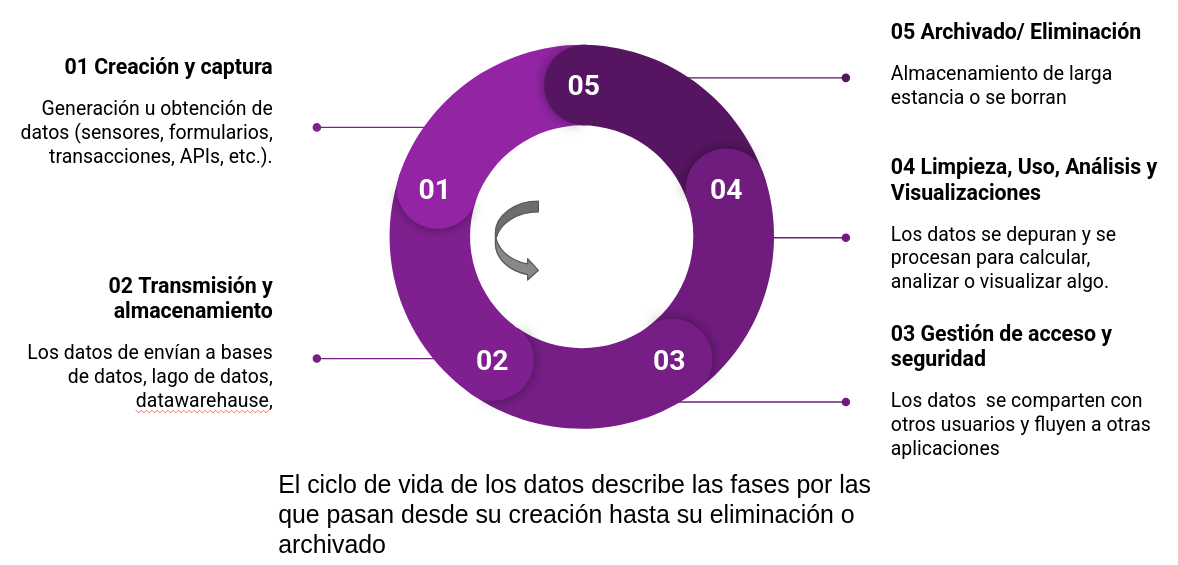
\includegraphics[width=\linewidth]{_fuentes/imagenes/ciclo_vida_completo}
    \column{0.4\textwidth}
      En la Parte I vimos captura y almacenamiento.
      \begin{block}{En esta clase (Parte II)}
        \textbf{03} Gesti\'on de acceso y seguridad.\\
        \textbf{04} Limpieza, uso, an\'alisis y visualizaci\'on.\\
        \textbf{05} Archivado y eliminaci\'on.
      \end{block}
  \end{columns}
\end{frame}

% ======================================================================
\section{Etapa 03: Gesti\'on de acceso y seguridad}

\begin{frame}{Acceso y seguridad: definici\'on y errores}
  \begin{columns}[t]
    \column{0.5\textwidth}
      \textbf{Definici\'on}\\[2pt]
      Los datos se comparten con otros usuarios y fluyen a otras aplicaciones;
      hay que protegerlos en el camino.
    \column{0.5\textwidth}
      \begin{block}{Posibles errores}
        \begin{itemize}
          \item Robo o secuestro de datos (ransomware).
          \item Datos inaccesibles; formatos obsoletos.
          \item Riesgos legales.
          \item Falta de encriptaci\'on o anonimizaci\'on.
          \item No cumplir con est\'andares.
        \end{itemize}
      \end{block}
  \end{columns}
\end{frame}

\begin{frame}{Ciberseguridad y amenazas potenciadas por IA}
  \textbf{Ciberseguridad}: pr\'acticas y principios para proteger sistemas y
  datos contra ataques digitales.
  \begin{columns}[t]
    \column{0.5\textwidth}
      \begin{block}{La IA como amenaza}
        \begin{itemize}
          \item Ingenier\'ia social (phishing).
          \item \textbf{Deepfakes} (audio/video falsos).
          \item \textbf{Data poisoning} (envenenar el entrenamiento).
          \item Password hacking acelerado.
        \end{itemize}
      \end{block}
    \column{0.5\textwidth}
      \begin{block}{La IA como defensa}
        \begin{itemize}
          \item Detecci\'on de fraude y phishing.
          \item Seguridad de red; detecci\'on m\'as r\'apida.
          \item Autenticaci\'on segura.
          \item Behavioral analytics.
        \end{itemize}
      \end{block}
  \end{columns}
\end{frame}

\begin{frame}{Riesgos en bases de datos y procesos ETL}
  \small
  \begin{center}
  \begin{tabular}{p{2.3cm} p{4.2cm} p{4.2cm}}
    \textbf{Riesgo} & \textbf{Bases de datos} & \textbf{Procesos ETL}\\[2pt]
    \hline
    Inyecci\'on & SQL Injection & Inyecci\'on en transformaciones\\[2pt]
    Exposici\'on & Datos en reposo & Datos en tr\'ansito\\[2pt]
    Autenticaci\'on & Privilegios excesivos & Credenciales en c\'odigo\\[2pt]
    Integridad & Corrupci\'on de datos & Datos no validados\\
    \hline
  \end{tabular}
  \end{center}
  \vspace{0.3em}
  Los datos se exponen en dos momentos: \textbf{en reposo} (guardados) y
  \textbf{en tr\'ansito} (mientras viajan). Ambos deben cifrarse.
\end{frame}

\begin{frame}{Buenas pr\'acticas de seguridad}
  \begin{itemize}
    \item \textbf{Inyecci\'on SQL}: usar \emph{consultas parametrizadas} y
          validar/sanitizar las entradas.
    \item \textbf{Cifrado}: en reposo (AES-256) y en tr\'ansito (TLS).
    \item \textbf{M\'inimos privilegios} (\emph{RBAC}, Role-Based Access
          Control): cada usuario solo accede a lo que necesita.
    \item \textbf{Hardening}: deshabilitar servicios y puertos innecesarios,
          cambiar credenciales por defecto.
    \item \textbf{Backups} autom\'aticos y encriptados, y \textbf{probarlos}.
  \end{itemize}
\end{frame}

\begin{frame}[fragile]{Inyecci\'on SQL: el ejemplo clasico}
\begin{lstlisting}[language=Python, basicstyle=\ttfamily\scriptsize]
# MAL: concatenar la entrada del usuario en la consulta
usuario = input()           # p.ej.:  ' OR '1'='1
q = "SELECT * FROM users WHERE name = '" + usuario + "'"
cur.execute(q)              # un atacante puede leer toda la tabla

# BIEN: consulta parametrizada (la entrada nunca es codigo)
cur.execute("SELECT * FROM users WHERE name = ?", (usuario,))
\end{lstlisting}
  La consulta parametrizada trata la entrada como \textbf{dato}, nunca como
  parte del comando SQL.
\end{frame}

% ======================================================================
\section{Etapa 04: Limpieza, an\'alisis y visualizaci\'on}

\begin{frame}{Limpieza y an\'alisis: definici\'on y errores}
  \begin{columns}[t]
    \column{0.5\textwidth}
      \textbf{Definici\'on}\\[2pt]
      Los datos se depuran y procesan para calcular, analizar o visualizar algo.
      \vspace{0.4em}
      \begin{block}{Taller de datos}
        Ordenar (tidy), buscar faltantes, describir y transformar tipos,
        visualizar y resolver problemas.
      \end{block}
    \column{0.5\textwidth}
      \begin{block}{Posibles errores}
        \begin{itemize}
          \item Uso de datos desactualizados.
          \item Interpretaci\'on incorrecta.
          \item Falta de revisi\'on de los procedimientos.
        \end{itemize}
      \end{block}
  \end{columns}
\end{frame}

\begin{frame}[fragile]{An\'alisis exploratorio de datos (EDA)}
  \begin{center}
  \begin{tikzpicture}[
      e/.style={rounded corners, draw=#1, very thick, fill=#1!15,
                minimum width=2.4cm, minimum height=1.2cm, align=center,
                font=\scriptsize\bfseries},
      every node/.style={align=center}]
    \node[e=molTeal]    (a) at (0,0)    {Analisis\\descriptivo};
    \node[e=molNaranja] (b) at (2.7,0)  {Tipos de\\variables};
    \node[e=molAmarillo](c) at (5.4,0)  {Datos\\faltantes};
    \node[e=molMorado]  (d) at (8.1,0)  {Outliers\\(atipicos)};
    \node[e=molAzul]    (f) at (10.8,0) {Correlacion\\de variables};
  \end{tikzpicture}
  \end{center}
  \vspace{0.3em}
  El \textbf{EDA} transforma datos en crudo en conclusiones: describe la
  distribuci\'on, ajusta tipos, trata faltantes, detecta at\'ipicos y mide
  relaciones. Para muchas variables se usa \textbf{reducci\'on de
  dimensionalidad} (PCA, t-SNE, UMAP).
\end{frame}

\begin{frame}[fragile]{Detectar outliers con el rango intercuartil (IQR)}
\begin{lstlisting}[language=Python]
q1 = df["ingreso"].quantile(0.25)
q3 = df["ingreso"].quantile(0.75)
iqr = q3 - q1
bajo, alto = q1 - 1.5 * iqr, q3 + 1.5 * iqr

# valores fuera de [bajo, alto] son atipicos
atipicos = df[(df["ingreso"] < bajo) | (df["ingreso"] > alto)]
\end{lstlisting}
  La regla \textbf{1.5 x IQR} marca como at\'ipicos los valores muy alejados del
  grueso de los datos; despu\'es se decide corregirlos, quitarlos o conservarlos.
\end{frame}

\begin{frame}{?`Por qu\'e SIEMPRE hay que visualizar?}
  \begin{columns}[c]
    \column{0.55\textwidth}
      El \textbf{cuarteto de Anscombe} (y el ``Datasaurus'') son conjuntos de
      datos con \textbf{las mismas estad\'isticas} -- igual media, varianza,
      correlaci\'on y recta de regresi\'on -- pero formas \textbf{completamente
      distintas}.
      \vspace{0.4em}
      \begin{block}{Moraleja}
        Las estad\'isticas resumen, pero pueden ocultar la realidad. Una gr\'afica
        revela patrones, outliers y errores que los n\'umeros esconden.
      \end{block}
    \column{0.45\textwidth}
      \begin{tikzpicture}[scale=0.9]
        % dos nubes con "misma" media pero forma distinta
        \draw[->,gray] (0,0)--(3.2,0); \draw[->,gray] (0,0)--(0,2.4);
        \foreach \x/\y in {0.4/0.4,0.8/0.7,1.2/1.0,1.6/1.3,2.0/1.6,2.4/1.9}
          {\fill[molTeal] (\x,\y) circle (1.6pt);}
        \node[font=\scriptsize] at (1.6,-0.35) {lineal};
        \begin{scope}[xshift=0cm,yshift=-3cm]
          \draw[->,gray] (0,0)--(3.2,0); \draw[->,gray] (0,0)--(0,2.4);
          \foreach \x/\y in {0.4/0.5,0.8/1.3,1.2/1.8,1.6/2.0,2.0/1.7,2.4/0.6}
            {\fill[molNaranja] (\x,\y) circle (1.6pt);}
          \node[font=\scriptsize] at (1.6,-0.35) {curva};
        \end{scope}
      \end{tikzpicture}
  \end{columns}
\end{frame}

% ======================================================================
\section{Etapa 05: Archivado y eliminaci\'on}

\begin{frame}{Archivado y eliminaci\'on: definici\'on y errores}
  \begin{columns}[t]
    \column{0.5\textwidth}
      \textbf{Definici\'on}\\[2pt]
      Almacenamiento de larga estancia para datos inactivos, o eliminaci\'on
      cuando ya no se necesitan.
      \vspace{0.4em}
      \begin{block}{?`Cu\'ando archivar?}
        Cuando los datos est\'an inactivos pero a\'un se necesitan para
        cumplimiento o an\'alisis hist\'orico.
      \end{block}
    \column{0.5\textwidth}
      \begin{block}{Posibles errores}
        \begin{itemize}
          \item Archivado inaccesible.
          \item Eliminaci\'on de datos por error.
          \item Incumplimiento de regulaciones.
        \end{itemize}
      \end{block}
  \end{columns}
\end{frame}

\begin{frame}{Buenas pr\'acticas y herramientas de archivado}
  \begin{columns}[t]
    \column{0.42\textwidth}
      \textbf{Mejores pr\'acticas}
      \begin{itemize}
        \item Mover a almacenamiento \textbf{fr\'io} (Glacier, Azure Blob
              Archive).
        \item Comprimir y cifrar antes de archivar.
        \item Documentar metadatos (fecha, responsable, raz\'on).
        \item Automatizar el proceso.
      \end{itemize}
    \column{0.58\textwidth}
      \scriptsize
      \begin{tabular}{p{2.2cm} p{1.6cm} p{2.6cm}}
        \textbf{Herramienta} & \textbf{Tipo} & \textbf{Uso tipico}\\[2pt]
        \hline
        AWS Glacier & Cloud & Archivado masivo en nube\\[2pt]
        MinIO & On-prem & Reemplazo de S3 on-premise\\[2pt]
        Veritas E. Vault & On-prem & Corporativo con cumplimiento\\[2pt]
        Archivematica & On-prem & Preservaci\'on a largo plazo\\[2pt]
        PostgreSQL part. & On-prem & Tablas muy grandes\\
        \hline
      \end{tabular}
  \end{columns}
\end{frame}

\begin{frame}{Cumplimiento legal y derechos ARCO}
  \begin{columns}[t]
    \column{0.5\textwidth}
      \begin{block}{Regulaciones clave}
        \begin{itemize}
          \item \textbf{GDPR}: derecho al olvido (Art. 17).
          \item \textbf{CCPA}: eliminaci\'on bajo solicitud.
          \item \textbf{HIPAA}: retenci\'on de registros m\'edicos.
        \end{itemize}
      \end{block}
      Documentar \textbf{todo}: cu\'ando, c\'omo y por qu\'e se archivaron o
      eliminaron los datos (auditor\'ia).
    \column{0.5\textwidth}
      \begin{block}{Derechos ARCO}
        \begin{itemize}
          \item \textbf{A}cceso: saber qu\'e datos hay sobre m\'i.
          \item \textbf{R}ectificaci\'on: corregir datos inexactos.
          \item \textbf{C}ancelaci\'on: eliminar datos que ya no se necesitan.
          \item \textbf{O}posici\'on: negarse a cierto uso (p.ej. publicidad).
        \end{itemize}
      \end{block}
  \end{columns}
\end{frame}

\begin{frame}{Clasificaci\'on de datos}
  Antes de archivar o eliminar conviene \textbf{clasificar} los datos:
  \begin{itemize}
    \item \textbf{Sensibilidad}: personales, financieros, de salud.
    \item \textbf{Frecuencia de uso}: activos, inactivos, hist\'oricos.
    \item \textbf{Requisitos legales}: tiempos de retenci\'on obligatorios.
  \end{itemize}
  \vspace{0.3em}
  Herramientas de etiquetado (a menudo automatico): Apache Ranger, AWS Macie,
  OpenDLP, Microsoft Presidio.
\end{frame}

% ======================================================================
\section{Resumen}

\begin{frame}{Takeaways}
  \begin{itemize}
    \item \textbf{Seguridad (03)}: cifrar en reposo y en tr\'ansito, usar
          consultas parametrizadas y \textbf{m\'inimos privilegios} (RBAC); la
          IA es a la vez amenaza (deepfakes, data poisoning) y defensa.
    \item \textbf{An\'alisis (04)}: el \textbf{EDA} describe, limpia faltantes,
          detecta outliers (IQR) y mide correlaciones.
    \item \textbf{Visualizar siempre}: Anscombe muestra que las mismas
          estad\'isticas pueden esconder formas muy distintas.
    \item \textbf{Archivado (05)}: almacenamiento fr\'io, comprimir/cifrar y
          documentar metadatos; eliminar cumpliendo \textbf{GDPR/ARCO}.
    \item Clasificar los datos por sensibilidad guia c\'omo protegerlos,
          archivarlos y eliminarlos.
  \end{itemize}
\end{frame}

\begin{frame}[plain]
  \molinaBanner
  \vfill
  \begin{center}
    {\color{molMorado}\Large\bfseries Gracias}\\[0.4em]
    {\color{molTeal} El ciclo de vida completo: de la captura a la eliminaci\'on}
  \end{center}
  \vfill\vspace{1.0cm}
  \molinaLogos
\end{frame}

\end{document}
